%UNDERSTANDING VOLUME - WORKSHEET 0 (IN-CLASS INSTRUCTION)
\documentclass[12pt, letterpaper, fleqn]{article}

% ----------------------------------------------------------
% PACKAGES
% ----------------------------------------------------------
\usepackage{graphicx}
\usepackage{xcolor}
\usepackage[most]{tcolorbox}
\usepackage{amsmath, amssymb}
\usepackage{fancyhdr}
\usepackage[utf8]{inputenc}
\usepackage[T1]{fontenc}
\usepackage{enumitem}
\usepackage{geometry}
\usepackage{tikz}
\usepackage{needspace}
\usepackage{multicol}

\usetikzlibrary{arrows.meta, calc, shapes.geometric}

% ----------------------------------------------------------
% PAGE SETUP
% ----------------------------------------------------------
\usepackage{times}
\geometry{letterpaper, top=1.25in, bottom=1.25in, marginpar=0.5in}

% ----------------------------------------------------------
% HEADER / FOOTER
% ----------------------------------------------------------
\newcommand{\logowidth}{3cm}
\setlength{\headheight}{20pt}
\setlength{\footskip}{40pt}

\pagestyle{fancy}
\fancyhf{}
\fancyhead[C]{\small\bfseries Understanding Volume}
\fancyfoot[L]{\raisebox{2pt}{
\includegraphics[width=\logowidth]{../kss.png}}}
\fancyfoot[C]{\thepage}
\fancyfoot[R]{5.18.0}

\renewcommand{\footrulewidth}{0.2pt}

% ----------------------------------------------------------
% THEME COLOR
% ----------------------------------------------------------
\definecolor{customteal}{HTML}{2fbdb9}

% ----------------------------------------------------------
% HELPER MACROS
% ----------------------------------------------------------
\newcommand{\blank}{\underline{\hspace{2.2cm}}}
\newcommand{\blanklong}{\underline{\hspace{6.5cm}}}
\newcommand{\blankshorter}{\underline{\hspace{1.5cm}}}

% ----------------------------------------------------------
% DOCUMENT
% ----------------------------------------------------------
\begin{document}

\textbf{Name:} \underline{\hspace{5cm}}
\hfill
\textbf{Date:} \underline{\hspace{3cm}}\\

\begin{tcolorbox}[colback=customteal!20]
    \large\textcolor{black}{\textbf{Introduction to Volume}}
\end{tcolorbox}

\vspace{3mm}
\noindent
**Volume** is the amount of 3D space an object takes up.
We measure volume in **unit cubes** (cubic units, e.g., cubic inches, cubic centimeters).
\begin{itemize}
    \item A single unit cube has a volume of $1\text{ cubic unit}$.
    \item We can find the volume of a rectangular prism by counting the number of unit cubes it takes to pack it without gaps.
\end{itemize}

\begin{center}
\begin{tikzpicture}[scale=0.8, line join=round]
% Draw a 2x2x2 cube stack
\foreach \x in {0,1} {
  \foreach \y in {0,1} {
    \foreach \z in {0,1} {
      \draw[fill=customteal!20, thick] (\x-\z*0.4, \y-\z*0.4) -- (\x+1-\z*0.4, \y-\z*0.4) -- (\x+1-\z*0.4, \y+1-\z*0.4) -- (\x-\z*0.4, \y+1-\z*0.4) -- cycle;
      \draw[fill=customteal!30, thick] (\x+1-\z*0.4, \y-\z*0.4) -- (\x+1.4-\z*0.4, \y+0.4-\z*0.4) -- (\x+1.4-\z*0.4, \y+1.4-\z*0.4) -- (\x+1-\z*0.4, \y+1-\z*0.4) -- cycle;
      \draw[fill=customteal!10, thick] (\x-\z*0.4, \y+1-\z*0.4) -- (\x+0.4-\z*0.4, \y+1.4-\z*0.4) -- (\x+1.4-\z*0.4, \y+1.4-\z*0.4) -- (\x+1-\z*0.4, \y+1-\z*0.4) -- cycle;
    }
  }
}
\end{tikzpicture}
\end{center}

\newpage
\begin{tcolorbox}[colback=customteal!20]
    \large\textcolor{black}{\textbf{Guided Practice}}
\end{tcolorbox}

\vspace{5mm}
\begin{enumerate}[itemsep=3cm, leftmargin=0.6cm]
\item How many unit cubes are in the 3D block shown in the model above?
\\
Answer: \blank cubes

\item If a box is packed with 3 layers of unit cubes, and each layer has 8 cubes, what is the total volume of the box?
\\
Equation: \blank $\times$ \blank $=$ \blank cubic units
\end{enumerate}

\end{document}
